%%%% Paramétrage du cours %%%%
\def\xxactivite{Cours}
\def\xxauteur{\textsl{Xavier Pessoles}}

\fichefalse
\proftrue
\tdfalse
\courstrue

\def\xxnumchapitre{Chapitre 1 \vspace{.2cm}}
\def\xxchapitre{\hspace{.12cm} Introduction}

\def\xxcompetences{%
\textsl{%
\textbf{Savoirs et compétences :}\\
\begin{itemize}[label=\ding{112},font=\color{ocre}] 
\item A voir
%\item \textit{Mod2.C17} : torseur dynamique
%\item \textit{Mod2.C17.SF1} : déterminer le torseur dynamique d’un solide, ou d’un ensemble de solides, par rapport à un autre solide
%\item \textit{Mod2.C15} : matrice d'inertie
%\item \textit{Res1.C2} : principe fondamental de la dynamique
%\item \textit{Res1.C1.SF1} : proposer une démarche permettant la détermination de la loi de mouvement
%\item \textit{Res1.C2.SF1} : proposer une méthode permettant la détermination d’une inconnue de liaison
\end{itemize}
}}



\def\xxfigures{
}%figues de la page de garde

\iflivret
\pagestyle{empty}


%%%%%%%% PAGE DE GARDE COURS
\ifcours
% ==== BANDEAU DES TITRES ==== 
\begin{tikzpicture}[remember picture,overlay]
\node at (current page.north west)
{\begin{tikzpicture}[remember picture,overlay]
\node[anchor=north west,inner sep=0pt] at (0,0) {\includegraphics[width=\paperwidth]{\thechapterimage}};
\draw[anchor=west] (-2cm,-8cm) node [line width=2pt,rounded corners=15pt,draw=ocre,fill=white,fill opacity=0.6,inner sep=40pt]{\strut\makebox[22cm]{}};
\draw[anchor=west] (1cm,-8cm) node {\huge\sffamily\bfseries\color{black} %
\begin{minipage}{1cm}
\rotatebox{90}{\LARGE\sffamily\textsc{\color{ocre}\textbf{\xxnumpartie}}}
\end{minipage} \hfill
\begin{minipage}[c]{14cm}
\begin{titrepartie}
\begin{flushright}
\renewcommand{\baselinestretch}{1.1} 
\Large\sffamily\textsc{\textbf{\xxpartie}}
\renewcommand{\baselinestretch}{1} 
\end{flushright}
\end{titrepartie}
\end{minipage} \hfill
\begin{minipage}[c]{3.5cm}
{\large\sffamily\textsc{\textbf{\color{ocre} \discipline}}}
\end{minipage} 
 };
\end{tikzpicture}};
\end{tikzpicture}
% ==== FIN BANDEAU DES TITRES ==== 


% ==== ONGLET 
\begin{tikzpicture}[overlay]
\node[shape=rectangle, 
      rounded corners = .25 cm,
	  draw= ocre,
	  line width=2pt, 
	  fill = ocre!10,
	  minimum width  = 2.5cm,
	  minimum height = 3cm,] at (18.3cm,0) {};
\node at (17.7cm,0) {\rotatebox{90}{\textbf{\Large\color{ocre}{\classe}}}};
%{};
\end{tikzpicture}
% ==== FIN ONGLET 


\vspace{3.5cm}

\begin{tikzpicture}[remember picture,overlay]
\draw[anchor=west] (-2cm,-6cm) node {\huge\sffamily\bfseries\color{black} %
\begin{minipage}{2cm}
\begin{center}
\LARGE\sffamily\textsc{\color{ocre}\textbf{\xxactivite}}
\end{center}
\end{minipage} \hfill
\begin{minipage}[c]{15cm}
\begin{titrechapitre}
\renewcommand{\baselinestretch}{1.1} 
\Large\sffamily\textsc{\textbf{\xxnumchapitre}}

\Large\sffamily\textsc{\textbf{\xxchapitre}}
\vspace{.5cm}

\renewcommand{\baselinestretch}{1} 
\normalsize\normalfont
\xxcompetences
\end{titrechapitre}
\end{minipage}  };
\end{tikzpicture}
\vfill

\begin{flushright}
\begin{minipage}[c]{.3\linewidth}
\begin{center}
\xxfigures
\end{center}
\end{minipage}\hfill
\begin{minipage}[c]{.6\linewidth}
\startcontents
%\printcontents{}{1}{}
\printcontents{}{1}{}
\end{minipage}
\end{flushright}

\begin{tikzpicture}[remember picture,overlay]
\draw[anchor=west] (4.5cm,-.7cm) node {
\begin{minipage}[c]{.2\linewidth}
\begin{flushright}

\includegraphics[width=2cm]{logoCC}
\end{flushright}
\end{minipage}
\begin{minipage}[c]{.2\linewidth}
\textsl{\xxauteur} \\
\textsl{\classe}
\end{minipage}
 };
\end{tikzpicture}

\newpage
\pagestyle{fancy}

%\newpage
%\pagestyle{fancy}

\else
\fi
%% FIN PAGE DE GARDE DES COURS

%%%%%%%% PAGE DE GARDE TD
\iftd

% BANDEAU EXO
\iflivret % SI LIVRET ET TD
\begin{tikzpicture}[remember picture,overlay]
\draw[anchor=west] (-2cm,-3.3cm) node {\huge\sffamily\bfseries\color{black} %
\begin{minipage}{5cm}
\begin{center}
\LARGE\sffamily\color{ocre}\textbf{\textsc{\xxactivite}}

\begin{center}
\xxfigures
\end{center}

\end{center}
\end{minipage} \hfill
\begin{minipage}[c]{12cm}
\begin{titrechapitre}
\renewcommand{\baselinestretch}{1.1} 
\large\sffamily\textbf{\textsc{\xxtitreexo}}

\small\sffamily{\textbf{\textit{\color{black!70}\xxsourceexo}}}
\vspace{.5cm}

\renewcommand{\baselinestretch}{1} 
\normalsize\normalfont
\xxcompetences
\end{titrechapitre}
\end{minipage}};
\end{tikzpicture}
\else % ELSE NOT LIVRET
\begin{tikzpicture}[remember picture,overlay]
\draw[anchor=west] (-2cm,-3.5cm) node {\huge\sffamily\bfseries\color{black} %
\begin{minipage}{5cm}
\begin{center}
\LARGE\sffamily\color{ocre}\textbf{\textsc{\xxactivite}}

\begin{center}
\xxfigures
\end{center}

\end{center}
\end{minipage} \hfill
\begin{minipage}[c]{12cm}
\begin{titrechapitre}
\renewcommand{\baselinestretch}{1.1} 
\large\sffamily\textbf{\textsc{\xxtitreexo}}

\small\sffamily{\textbf{\textit{\color{black!70}\xxsourceexo}}}
\vspace{.5cm}

\renewcommand{\baselinestretch}{1} 
\normalsize\normalfont
\xxcompetences
\end{titrechapitre}
\end{minipage}};
\end{tikzpicture}

\fi

\else   % FIN IF TD
\fi


%%%%%%%% PAGE DE GARDE FICHE
\iffiche
\begin{tikzpicture}[remember picture,overlay]
\node at (current page.north west)
{\begin{tikzpicture}[remember picture,overlay]
\draw[anchor=west] (-2cm,\xxYCartouche) node [line width=2pt,rounded corners=15pt,draw=ocre,fill=white,fill opacity=0.6,inner sep=40pt]{\strut\makebox[22cm]{}};
\draw[anchor=west] (1cm,\xxYCartouche) node {\huge\sffamily\bfseries\color{black} %
\begin{minipage}{1cm}
\rotatebox{90}{\LARGE\sffamily\textsc{\color{ocre}\textbf{\xxnumpartie}}}
\end{minipage} \hfill
\begin{minipage}[c]{14cm}
\begin{titrepartie}
\begin{flushright}
\renewcommand{\baselinestretch}{1.1} 
\large\sffamily\textsc{\textbf{\xxpartie} \\} 

\vspace{.2cm}

\normalsize\sffamily\textsc{\textbf{\xxnumchapitre -- \xxchapitre}}
\renewcommand{\baselinestretch}{1} 
\end{flushright}
\end{titrepartie}
\end{minipage} \hfill
\begin{minipage}[c]{3.5cm}
{\large\sffamily\textsc{\textbf{\color{ocre} \discipline}}}
\end{minipage} 
 };
\end{tikzpicture}};
\end{tikzpicture}

\iflivret % SI LIVRET
\begin{tikzpicture}[overlay]
\node[shape=rectangle, 
      rounded corners = .25 cm,
	  draw= ocre,
	  line width=2pt, 
	  fill = ocre!10,
	  minimum width  = 2.5cm,
	  minimum height = 2.5cm,] at (18.5cm,\xxYongletGarde) {};
\node at (17.9cm,\xxYongletGarde) {\rotatebox{90}{\textsf{\textbf{\large\color{ocre}{\classe}}}}};
%{};
\end{tikzpicture}
\else  % SI PAS LIVRET
\iftd %% SI TD et PAS LIVRET
\begin{tikzpicture}[overlay]
\node[shape=rectangle, 
      rounded corners = .25 cm,
	  draw= ocre,
	  line width=2pt, 
	  fill = ocre!10,
	  minimum width  = 2.5cm,
	  minimum height = 2.5cm,] at (18.6cm,\xxYOnget) {}; %% 0.9 par défaut
\node at (18cm,\xxYOnget) {\rotatebox{90}{\textsf{\textbf{\large\color{ocre}{\classe}}}}};
%{};
\end{tikzpicture}

\else % FIN DU SI TD PAS LIVRET 
\begin{tikzpicture}[overlay]
\node[shape=rectangle, 
      rounded corners = .25 cm,
	  draw= ocre,
	  line width=2pt, 
	  fill = ocre!10,
	  minimum width  = 2.5cm,
%	  minimum height = 2.5cm,] at (18.5cm,1.1cm) {}; % \xxYOnget 0.5
	  minimum height = 2.5cm,] at (18.6cm,.5cm) {};
\node at (18cm,.5cm) {\rotatebox{90}{\textsf{\textbf{\large\color{ocre}{\classe}}}}};
%{};
\end{tikzpicture}
\fi
\fi
\else
\fi



\else
\pagestyle{empty}


%%%%%%%% PAGE DE GARDE COURS
\ifcours
% ==== BANDEAU DES TITRES ==== 
\begin{tikzpicture}[remember picture,overlay]
\node at (current page.north west)
{\begin{tikzpicture}[remember picture,overlay]
\node[anchor=north west,inner sep=0pt] at (0,0) {\includegraphics[width=\paperwidth]{\thechapterimage}};
\draw[anchor=west] (-2cm,-8cm) node [line width=2pt,rounded corners=15pt,draw=ocre,fill=white,fill opacity=0.6,inner sep=40pt]{\strut\makebox[22cm]{}};
\draw[anchor=west] (1cm,-8cm) node {\huge\sffamily\bfseries\color{black} %
\begin{minipage}{1cm}
\rotatebox{90}{\LARGE\sffamily\textsc{\color{ocre}\textbf{\xxnumpartie}}}
\end{minipage} \hfill
\begin{minipage}[c]{14cm}
\begin{titrepartie}
\begin{flushright}
\renewcommand{\baselinestretch}{1.1} 
\Large\sffamily\textsc{\textbf{\xxpartie}}
\renewcommand{\baselinestretch}{1} 
\end{flushright}
\end{titrepartie}
\end{minipage} \hfill
\begin{minipage}[c]{3.5cm}
{\large\sffamily\textsc{\textbf{\color{ocre} \discipline}}}
\end{minipage} 
 };
\end{tikzpicture}};
\end{tikzpicture}
% ==== FIN BANDEAU DES TITRES ==== 


% ==== ONGLET 
\begin{tikzpicture}[overlay]
\node[shape=rectangle, 
      rounded corners = .25 cm,
	  draw= ocre,
	  line width=2pt, 
	  fill = ocre!10,
	  minimum width  = 2.5cm,
	  minimum height = 3cm,] at (18.3cm,0) {};
\node at (17.7cm,0) {\rotatebox{90}{\textbf{\Large\color{ocre}{\classe}}}};
%{};
\end{tikzpicture}
% ==== FIN ONGLET 


\vspace{3.5cm}

\begin{tikzpicture}[remember picture,overlay]
\draw[anchor=west] (-2cm,-6cm) node {\huge\sffamily\bfseries\color{black} %
\begin{minipage}{2cm}
\begin{center}
\LARGE\sffamily\textsc{\color{ocre}\textbf{\xxactivite}}
\end{center}
\end{minipage} \hfill
\begin{minipage}[c]{15cm}
\begin{titrechapitre}
\renewcommand{\baselinestretch}{1.1} 
\Large\sffamily\textsc{\textbf{\xxnumchapitre}}

\Large\sffamily\textsc{\textbf{\xxchapitre}}
\vspace{.5cm}

\renewcommand{\baselinestretch}{1} 
\normalsize\normalfont
\xxcompetences
\end{titrechapitre}
\end{minipage}  };
\end{tikzpicture}
\vfill

\begin{flushright}
\begin{minipage}[c]{.3\linewidth}
\begin{center}
\xxfigures
\end{center}
\end{minipage}\hfill
\begin{minipage}[c]{.6\linewidth}
\startcontents
%\printcontents{}{1}{}
\printcontents{}{1}{}
\end{minipage}
\end{flushright}

\begin{tikzpicture}[remember picture,overlay]
\draw[anchor=west] (4.5cm,-.7cm) node {
\begin{minipage}[c]{.2\linewidth}
\begin{flushright}

\includegraphics[width=2cm]{logoCC}
\end{flushright}
\end{minipage}
\begin{minipage}[c]{.2\linewidth}
\textsl{\xxauteur} \\
\textsl{\classe}
\end{minipage}
 };
\end{tikzpicture}

\newpage
\pagestyle{fancy}

%\newpage
%\pagestyle{fancy}

\else
\fi
%% FIN PAGE DE GARDE DES COURS

%%%%%%%% PAGE DE GARDE TD
\iftd

% BANDEAU EXO
\iflivret % SI LIVRET ET TD
\begin{tikzpicture}[remember picture,overlay]
\draw[anchor=west] (-2cm,-3.3cm) node {\huge\sffamily\bfseries\color{black} %
\begin{minipage}{5cm}
\begin{center}
\LARGE\sffamily\color{ocre}\textbf{\textsc{\xxactivite}}

\begin{center}
\xxfigures
\end{center}

\end{center}
\end{minipage} \hfill
\begin{minipage}[c]{12cm}
\begin{titrechapitre}
\renewcommand{\baselinestretch}{1.1} 
\large\sffamily\textbf{\textsc{\xxtitreexo}}

\small\sffamily{\textbf{\textit{\color{black!70}\xxsourceexo}}}
\vspace{.5cm}

\renewcommand{\baselinestretch}{1} 
\normalsize\normalfont
\xxcompetences
\end{titrechapitre}
\end{minipage}};
\end{tikzpicture}
\else % ELSE NOT LIVRET
\begin{tikzpicture}[remember picture,overlay]
\draw[anchor=west] (-2cm,-3.5cm) node {\huge\sffamily\bfseries\color{black} %
\begin{minipage}{5cm}
\begin{center}
\LARGE\sffamily\color{ocre}\textbf{\textsc{\xxactivite}}

\begin{center}
\xxfigures
\end{center}

\end{center}
\end{minipage} \hfill
\begin{minipage}[c]{12cm}
\begin{titrechapitre}
\renewcommand{\baselinestretch}{1.1} 
\large\sffamily\textbf{\textsc{\xxtitreexo}}

\small\sffamily{\textbf{\textit{\color{black!70}\xxsourceexo}}}
\vspace{.5cm}

\renewcommand{\baselinestretch}{1} 
\normalsize\normalfont
\xxcompetences
\end{titrechapitre}
\end{minipage}};
\end{tikzpicture}

\fi

\else   % FIN IF TD
\fi


%%%%%%%% PAGE DE GARDE FICHE
\iffiche
\begin{tikzpicture}[remember picture,overlay]
\node at (current page.north west)
{\begin{tikzpicture}[remember picture,overlay]
\draw[anchor=west] (-2cm,\xxYCartouche) node [line width=2pt,rounded corners=15pt,draw=ocre,fill=white,fill opacity=0.6,inner sep=40pt]{\strut\makebox[22cm]{}};
\draw[anchor=west] (1cm,\xxYCartouche) node {\huge\sffamily\bfseries\color{black} %
\begin{minipage}{1cm}
\rotatebox{90}{\LARGE\sffamily\textsc{\color{ocre}\textbf{\xxnumpartie}}}
\end{minipage} \hfill
\begin{minipage}[c]{14cm}
\begin{titrepartie}
\begin{flushright}
\renewcommand{\baselinestretch}{1.1} 
\large\sffamily\textsc{\textbf{\xxpartie} \\} 

\vspace{.2cm}

\normalsize\sffamily\textsc{\textbf{\xxnumchapitre -- \xxchapitre}}
\renewcommand{\baselinestretch}{1} 
\end{flushright}
\end{titrepartie}
\end{minipage} \hfill
\begin{minipage}[c]{3.5cm}
{\large\sffamily\textsc{\textbf{\color{ocre} \discipline}}}
\end{minipage} 
 };
\end{tikzpicture}};
\end{tikzpicture}

\iflivret % SI LIVRET
\begin{tikzpicture}[overlay]
\node[shape=rectangle, 
      rounded corners = .25 cm,
	  draw= ocre,
	  line width=2pt, 
	  fill = ocre!10,
	  minimum width  = 2.5cm,
	  minimum height = 2.5cm,] at (18.5cm,\xxYongletGarde) {};
\node at (17.9cm,\xxYongletGarde) {\rotatebox{90}{\textsf{\textbf{\large\color{ocre}{\classe}}}}};
%{};
\end{tikzpicture}
\else  % SI PAS LIVRET
\iftd %% SI TD et PAS LIVRET
\begin{tikzpicture}[overlay]
\node[shape=rectangle, 
      rounded corners = .25 cm,
	  draw= ocre,
	  line width=2pt, 
	  fill = ocre!10,
	  minimum width  = 2.5cm,
	  minimum height = 2.5cm,] at (18.6cm,\xxYOnget) {}; %% 0.9 par défaut
\node at (18cm,\xxYOnget) {\rotatebox{90}{\textsf{\textbf{\large\color{ocre}{\classe}}}}};
%{};
\end{tikzpicture}

\else % FIN DU SI TD PAS LIVRET 
\begin{tikzpicture}[overlay]
\node[shape=rectangle, 
      rounded corners = .25 cm,
	  draw= ocre,
	  line width=2pt, 
	  fill = ocre!10,
	  minimum width  = 2.5cm,
%	  minimum height = 2.5cm,] at (18.5cm,1.1cm) {}; % \xxYOnget 0.5
	  minimum height = 2.5cm,] at (18.6cm,.5cm) {};
\node at (18cm,.5cm) {\rotatebox{90}{\textsf{\textbf{\large\color{ocre}{\classe}}}}};
%{};
\end{tikzpicture}
\fi
\fi
\else
\fi



\fi
\setlength{\columnseprule}{.1pt}

\vspace{2cm}
\pagestyle{fancy}
\thispagestyle{plain}








\section{L'Intelligence Artificielle, qu'est ce que c'est, à quoi ça sert ?}

%\subsection{Première approche. Que veut-on ? Qu'obtient-on ?}
\begin{defi}[Intelligence Artificielle]
Wikipedia -- L'intelligence artificielle (IA) est « l'ensemble des théories et des techniques mises en œuvre en vue de réaliser des machines capables de simuler l'intelligence ». 
\end{defi}

En première approche, l'IA peut être assimilée à un ensemble d'algorithmes permettant de réaliser des tris, des classifications.
\begin{exemple}~\\
\\
\vspace{-1cm}

\begin{multicols}{2}
\begin{center}
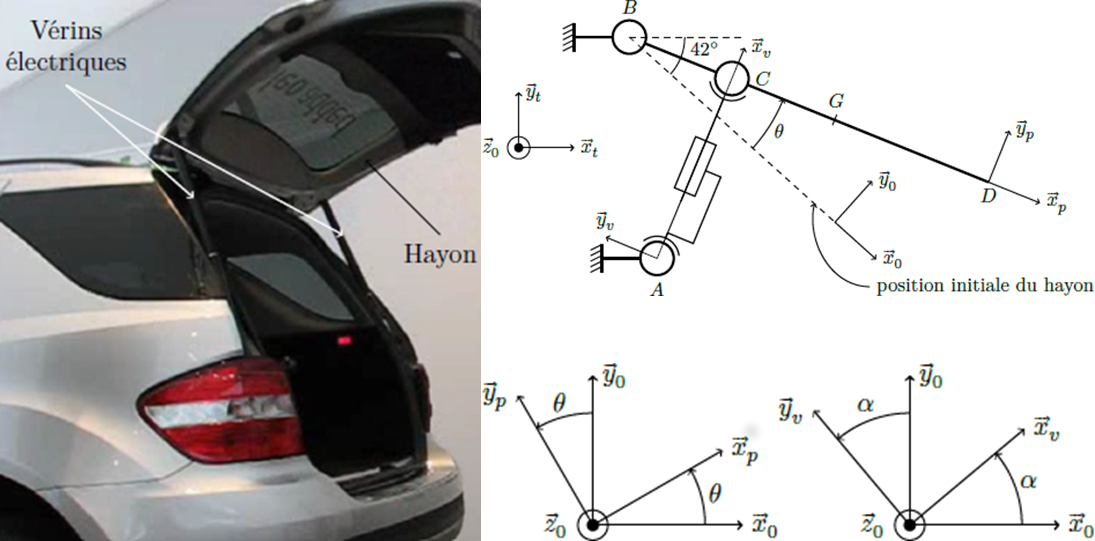
\includegraphics[width=.8\linewidth]{fig_01}
\end{center}
Identification d'objets, en temps réel, dans une vidéo.

\begin{center}
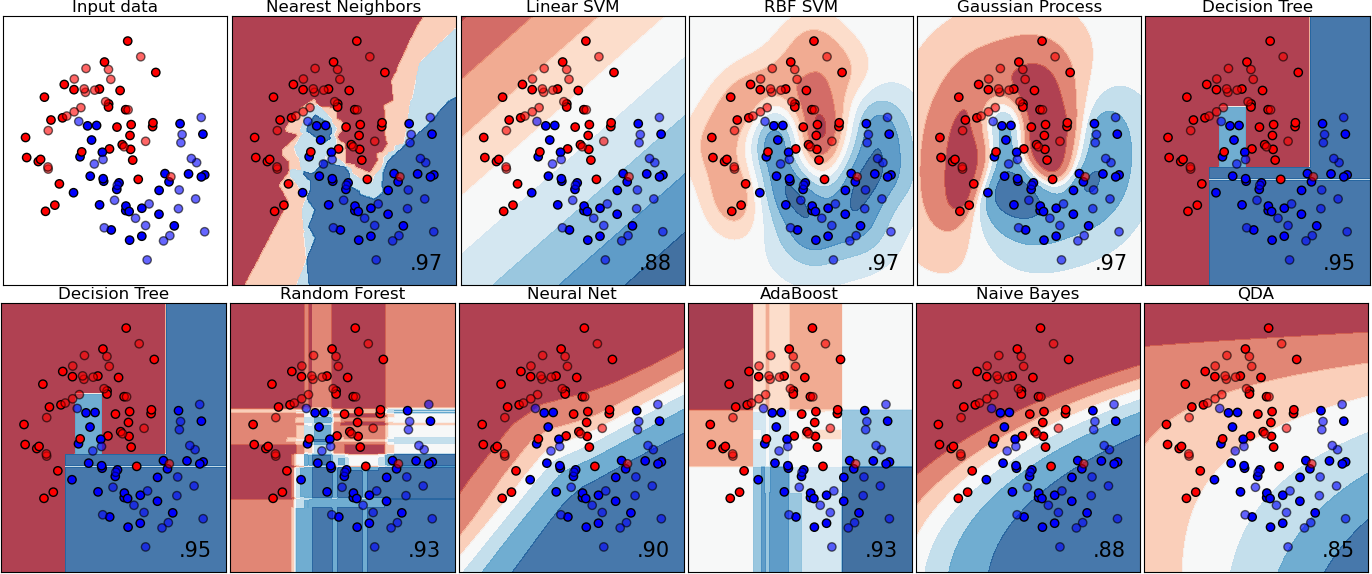
\includegraphics[width=.95\linewidth]{fig_02_a}
\end{center}


Comparaison du résultats d'algorithmes de classification permettant de classifier un nuage de points bleus et rouges de transparences différentes.
\end{multicols}

On remarquera sur l'exemple de gauche que l'algorithme parvient à identifier sur l'image des zones puis à identifier à quoi elles correspondent. On remarquera aussi que la flamme est identifiée comme étant un donut...


\begin{flushright}
\footnotesize
\url{exploring-opencvs-deep-learning-object-detection-library} \&  \url{https://scikit-learn.org/}.
\normalsize

\end{flushright}
\end{exemple}



Pour utiliser un algorithme d'IA il est nécessaire de disposer de données... en général beaucoup de données. 
\begin{defi}[Données]
Les données utilisées par un algorithme d'IA peuvent être sous différentes formes : 
\begin{itemize}
\item des données quantitatives continues qui peuvent prendre n'importe quelles valeurs dans un ensemble de valeurs (par exemple la température);
\item des données quantitatives discrètes qui peuvent prendre un nombre limité de valeurs dans un ensemble de valeurs (par exemple nombre de pièces d'un logement);
\item des données qualitatives (ordinales ou nominales suivant qu'on puissent les classer ou non, par exemple des couleurs, des notes à un test d'opinion ...).
\end{itemize}

\end{defi}

Pour pouvoir traiter ces données, il peut être nécessaire qu'elles soient organisées sous une certaine forme. On peut par exemple identifier : 
\begin{itemize}
\item les données structurées, dans une base de données par exemple;
\item les données semi-structurées, dans un fichier csv, xml ou json par exemple;
\item les données non structurées comme un image, du texte, ou une vidéo.
\end{itemize}

\begin{defi}[Observations -- Caractéristiques]

On appelle observation (ou individu ou objet) une << ligne de donnée >> qui va être utilisée par un algorithme d'apprentissage. 

Une observation est composée de caractéristiques qui varient pour chacun des observations. 
\end{defi}

\begin{exemple}~\\

\begin{minipage}[c]{.65\linewidth}
Dans le cas de la base de donnée des Iris, présente par exemple dans \texttt{scikit-learn}, les données sont composées de 150 observations, chacune composée de 4 caractéristiques : longueur et largeur du sépale ainsi que longueur et largeur du pétale.
\end{minipage} \hfill
\begin{minipage}[c]{.3\linewidth}
\begin{center}
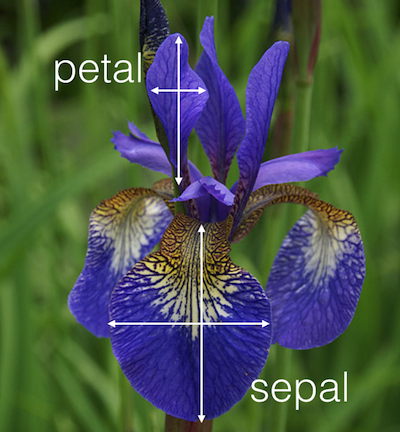
\includegraphics[width=.6\linewidth]{fig_10}
\end{center}
\end{minipage} 

\end{exemple}


\begin{defi}[Big data -- Wikipedia]
Mégadonnées ou données massives. Le big data désigne les ressources d’informations dont les caractéristiques en termes de volume, de vélocité et de variété imposent l’utilisation de technologies et de méthodes analytiques particulières pour générer de la valeur, et qui dépassent en général les capacités d'une seule et unique machine et nécessitent des traitements parallélisés.
\end{defi}


Que fait-on avec ces données ? En général les algorithmes vont chercher un lien entre ces données. Dans le cas où il existe un lien connu par le \textit{Data Scientist} on parle d'apprentissage supervisé. 

Si ce lien n'est pas connu, on parle d'apprentissage non supervisé ou de clustering. 




\begin{defi}[Apprentissage automatique -- Machine learning]
L'apprentissage automatique est un champ de l'intelligence artificielle dont l'objectif est d'analyser un grand volume de
données afin de déterminer des motifs et de réaliser un modèle prédictif. 

L'apprentissage comprend deux phases : 
\begin{itemize}
\item l’entraînement (ou apprentissage) est une phase d'estimation du modèle à partir de données d'observations; 
\item la mise en production du modèle est une phase pendant laquelle de nouvelles données sont traitées dans le but d'obtenir le résultat souhaité. 
\end{itemize}

L’entraînement peut être poursuivi même en phase de production.

\end{defi}


\begin{exemple}~\\

\begin{center}
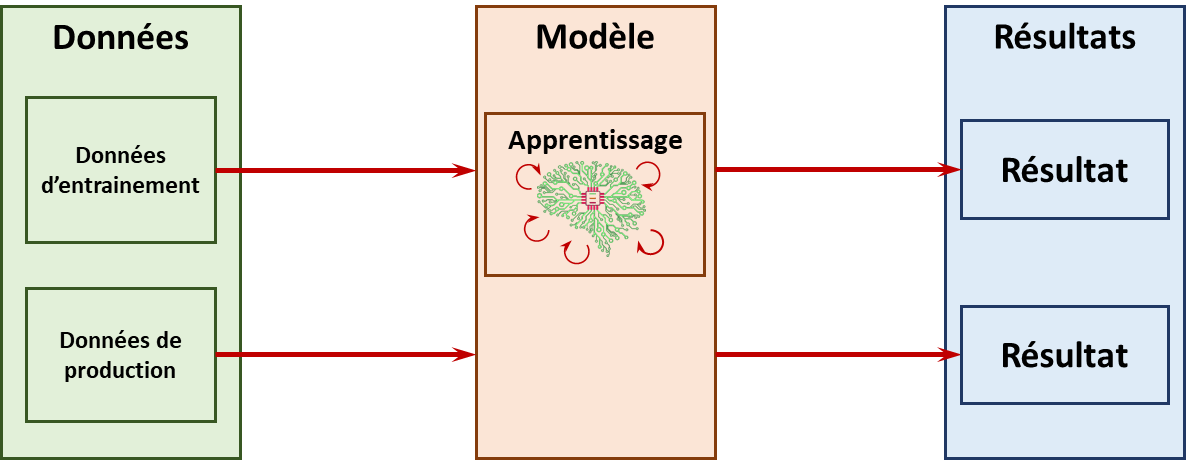
\includegraphics[width=.6\linewidth]{fig_05}
\end{center}
\end{exemple}


\begin{defi}[Apprentissage supervisé -- Induction]
Tâche d'apprentissage au cours duquel l'algorithme (ou fonction de prédiction) va, à partir d'un ensemble de données \textbf{étiquetées}, déterminer un lien entre un ensemble les données et les étiquettes. 

Dans un second temps, l'algorithme devra être capable de prédire l'étiquette (sans la connaître) à partir de données originales.

\end{defi}



\begin{exemple}~\\

\begin{center}
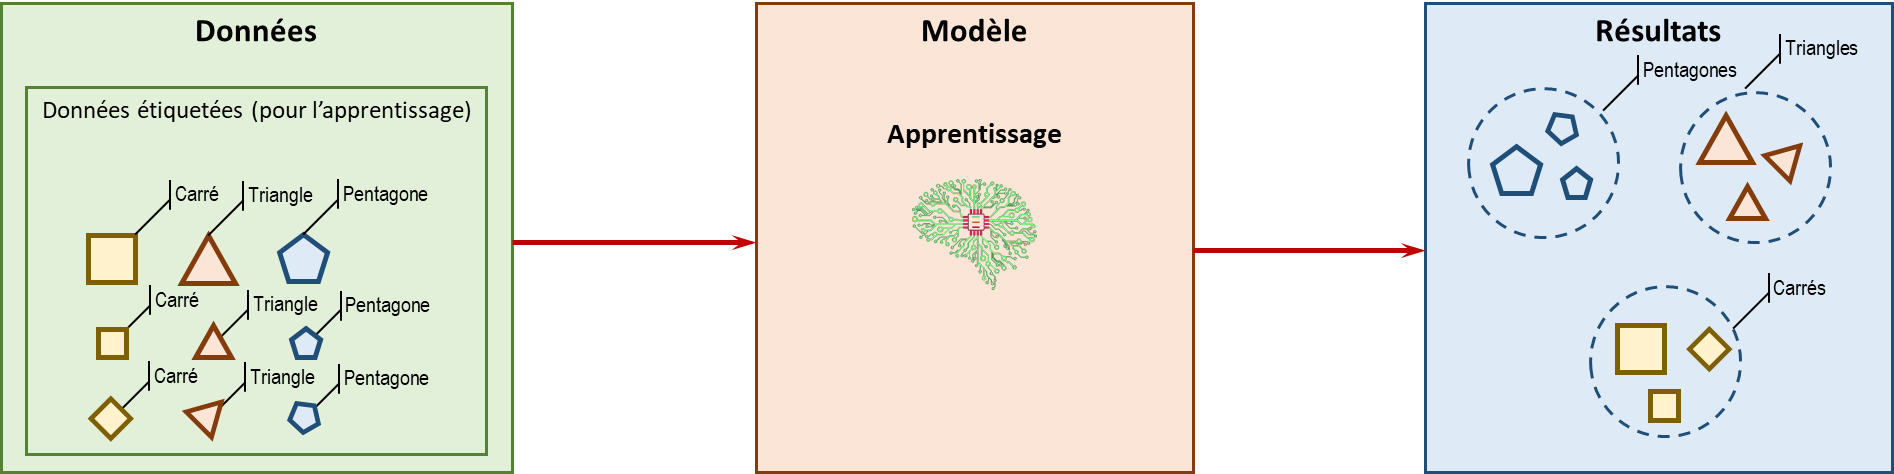
\includegraphics[width=.8\linewidth]{fig_06}
\end{center}
\end{exemple}


\begin{exemple}
Soit un ensemble d'images en noir et blanc représentant des chiffres de 0 à 9. L'algorithme doit dans un premier temps \textit{apprendre} le lien entre l'image et le chiffre. 
Dans un second temps, l'algorithme devra déterminer le chiffre en fonction d'une image seule.
\end{exemple}

\begin{defi}[Apprentissage non supervisé -- Clustering]
Tâche d'apprentissage au cours duquel l'algorithme (ou fonction de prédiction) va, à partir d'un ensemble de données \textbf{non étiquetées}, déterminer un lien entre les données (et les regrouper). 
\end{defi}



\begin{exemple} ~\\


\begin{center}
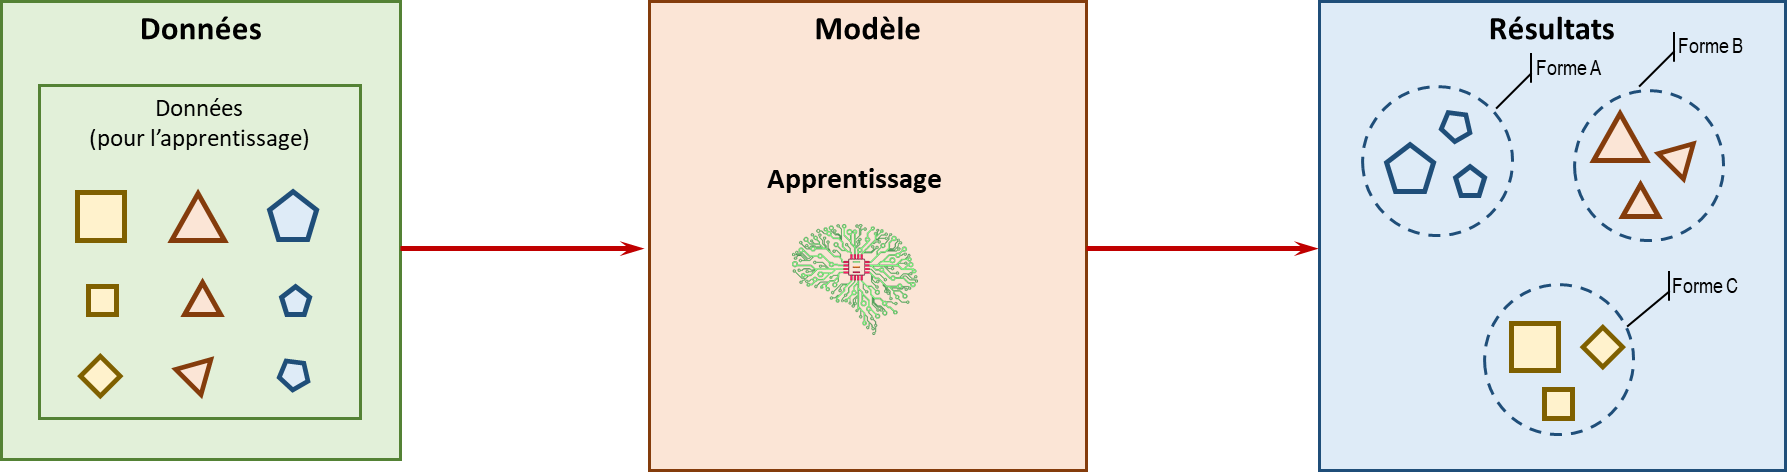
\includegraphics[width=.8\linewidth]{fig_07}
\end{center}


Classification d'iris en utilisant un algorithme d'apprentissage non supervisé.
\begin{center}
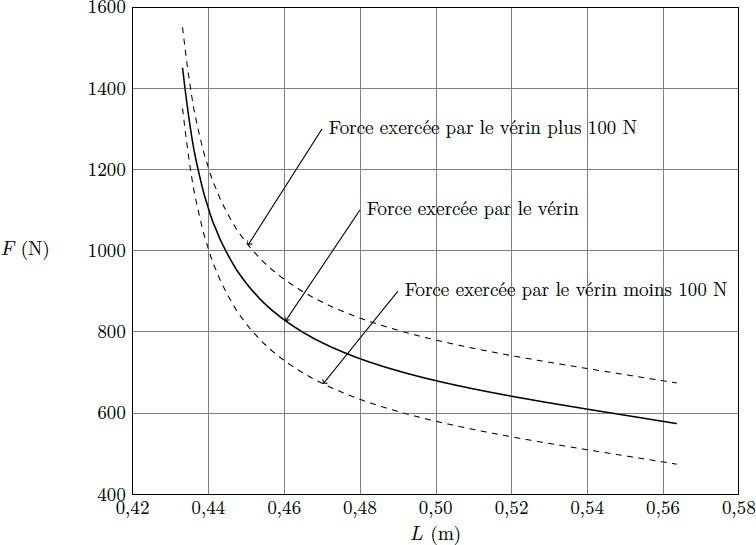
\includegraphics[width=.8\linewidth]{fig_03}
\end{center}

On remarque (lorsque l'image est en couleur) que sur des mesures sur 150 iris, l'algorithme a réussi à retrouver les 3 différentes espèces, sans les connaître, à 3 erreurs près.

\end{exemple}


\begin{defi}[Apprentissage par renforcement]
Si au cours de l'apprentissage supervisé, un mécanisme de récompense est mis en \oe{}uvre pour améliorer les performances du modèle, on parle d'apprentissage par renforcement.
\end{defi}



On peut donc faire une synthèse des méthodes d'apprentissage dont nous avons pris connaissance (il en existe d'autres).

\begin{center}
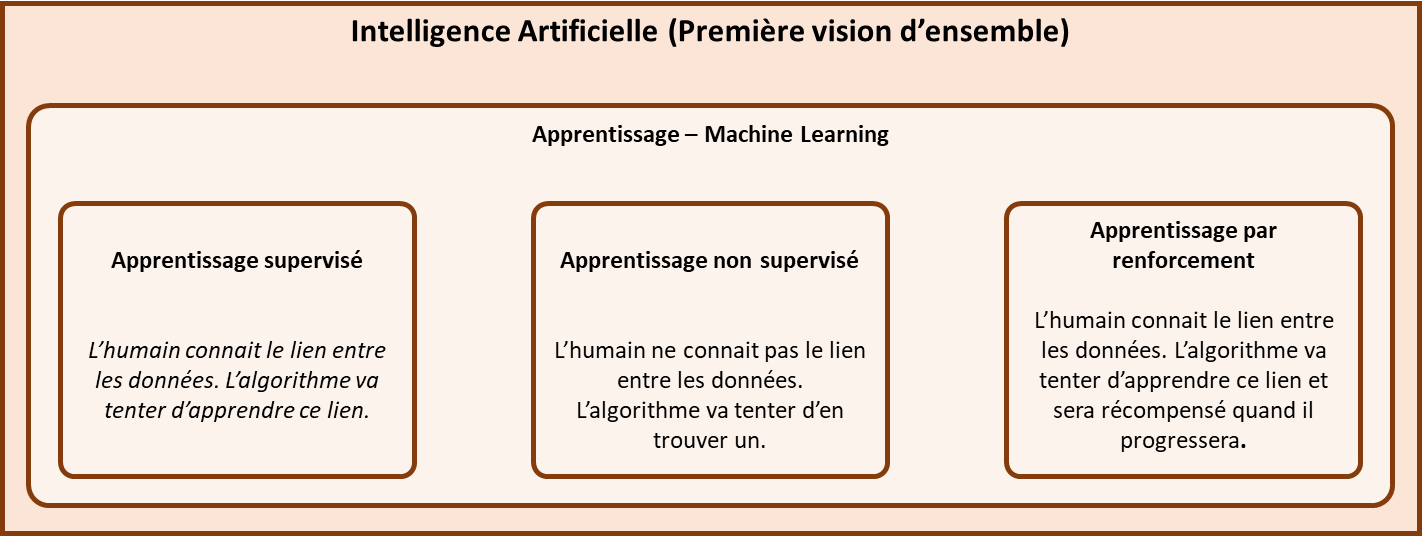
\includegraphics[width=.8\linewidth]{fig_08}
\end{center}

\textit{Comment situer le deep learning parmi ces méthodes d'apprentissage ? -- NDLR (ie XP) pour moi l'utilisation du terme << deep learning >> apparaît lorsqu'on commence à utiliser des réseaux de neurones... mais les réseaux de neurones peuvent être utilisés dans chacune des méthodes d'apprentissage sus-citées...}


\section{Mécanismes d'apprentissages}

\subsection{Classification des algorithmes d'apprentissage}

\begin{center}
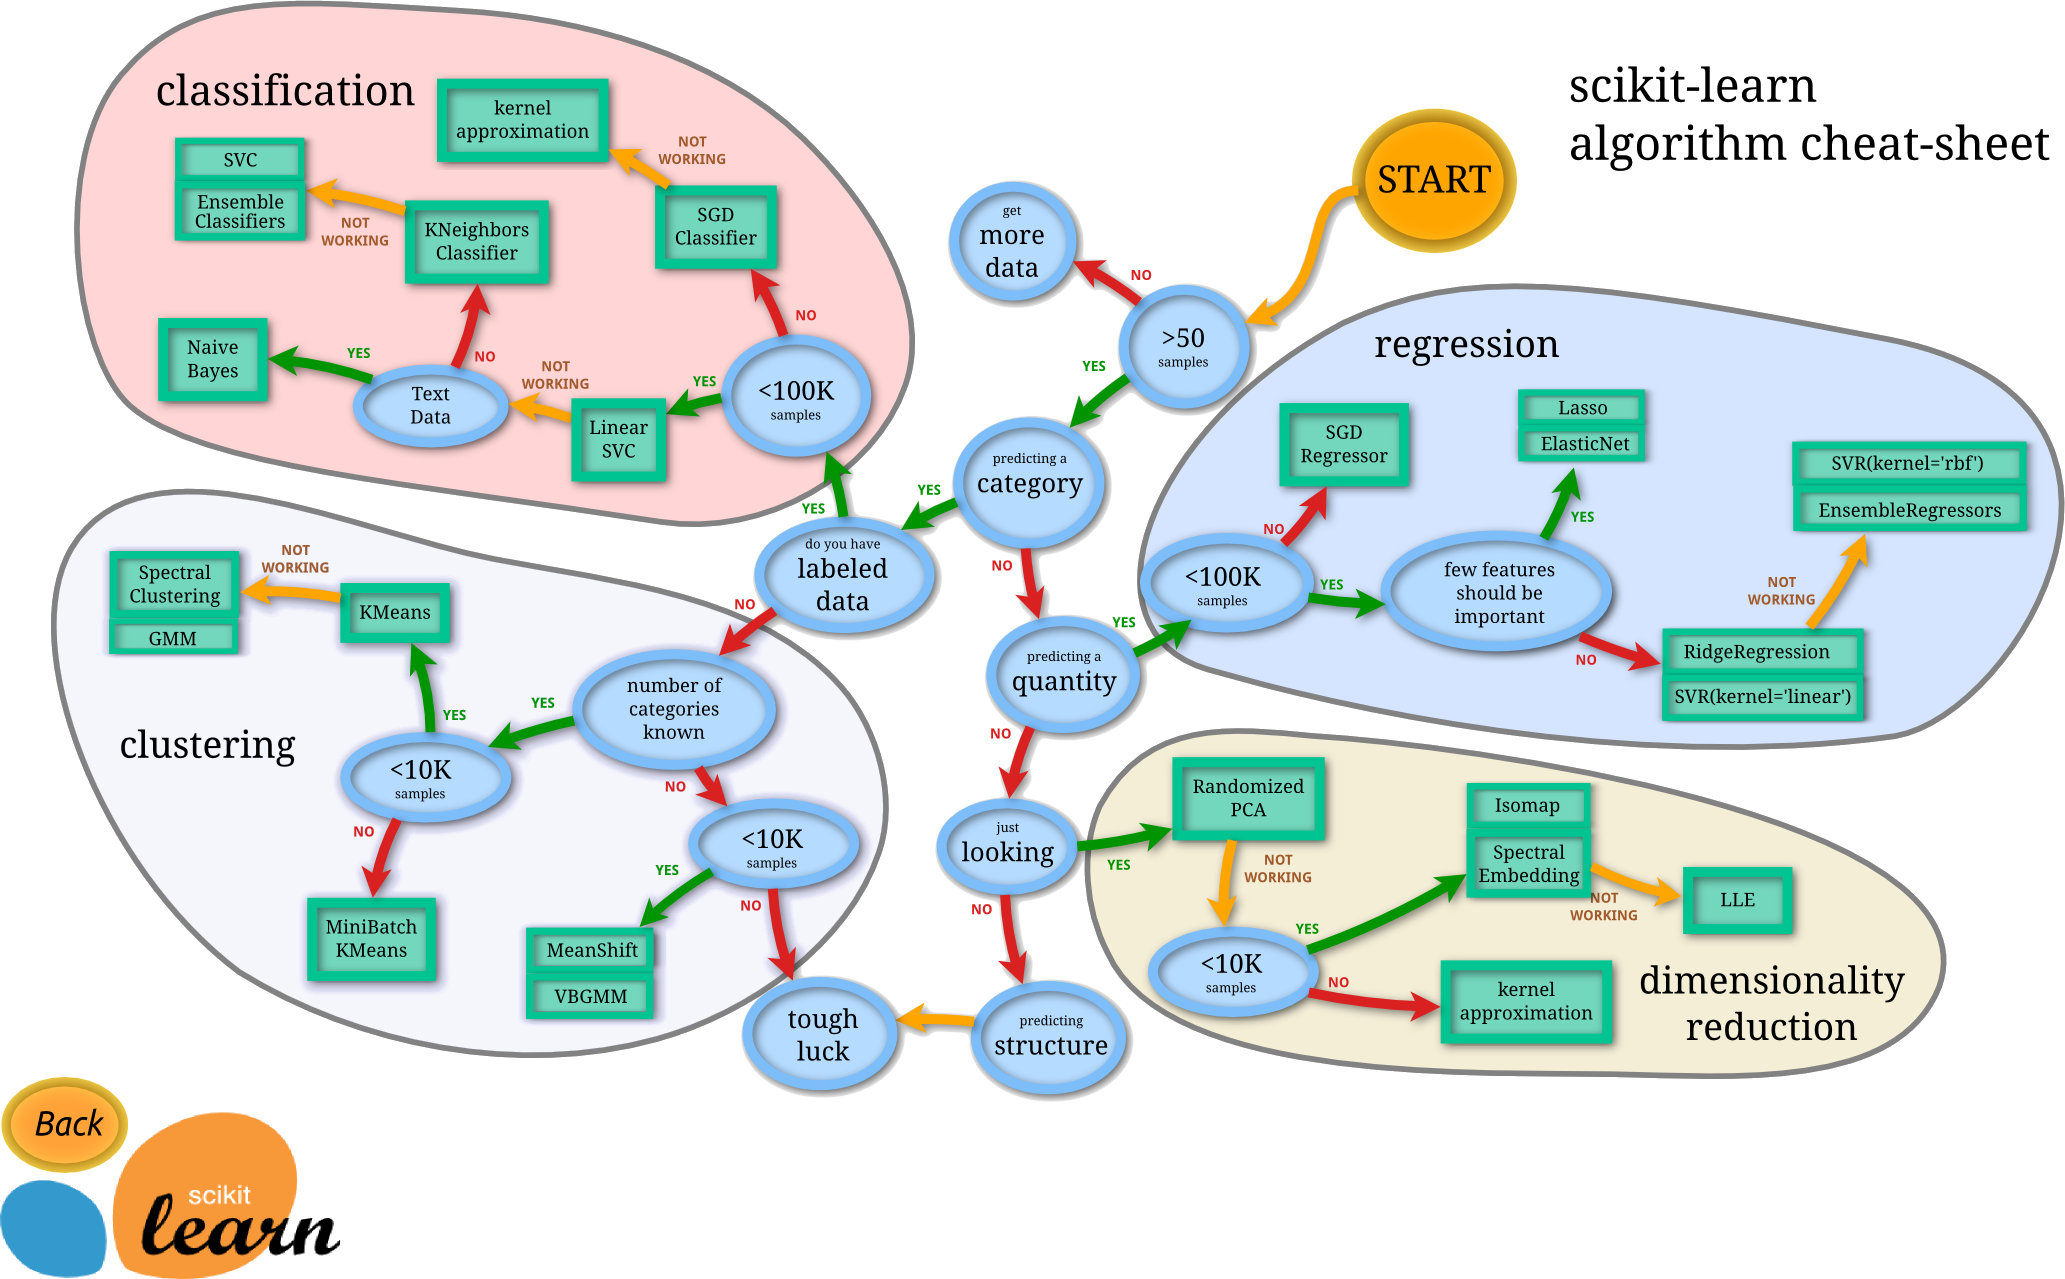
\includegraphics[width=\linewidth]{fig_09}
\end{center}

\subsection{Données et séparation des données/Gestion des données ?}
Lorsque l'on souhaite disposer d'un modèle défini par un algorithme d'IA, il faut en premier lieu disposer de données. 

\subsubsection{Cas de l'apprentissage supervisé}

En apprentissage supervisé, il est nécessaire de connaître des données d'entrées ainsi que les sorties correspondantes (appelées aussi \texttt{cibles} ou \texttt{target}).

Dans le cadre d'une programmation \texttt{Python} avec la bibliothèque \texttt{scikit-learn} les données d'entées et de sorties peuvent être implémentées en utilisant des \texttt{numpy.ndarray}.

Ainsi, si les données d'entrées, stockées dans la variable \texttt{data} sont composées de \texttt{n} observations elles mêmes composées de \texttt{p} catégories, le \text{shape} de \texttt{data} sera \texttt{(n,p)}.

La donnée cible sera quant à elle un vecteur de \texttt{n} valeurs. 

\begin{exemple}~\\
\begin{center}
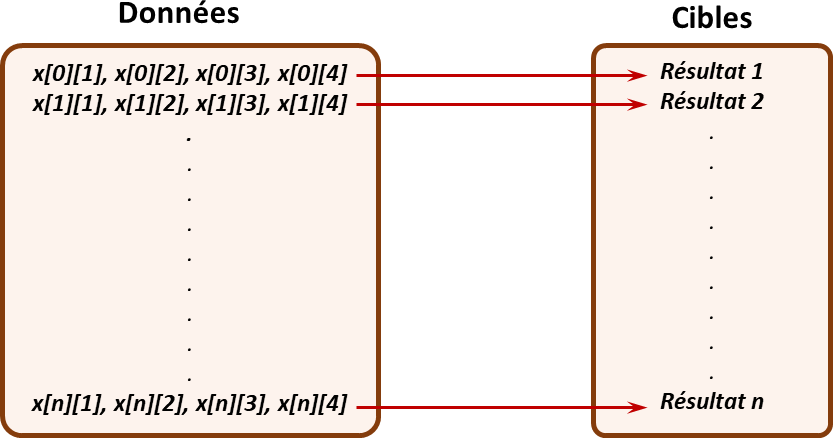
\includegraphics[width=.5\linewidth]{fig_11}
\end{center}
\end{exemple}

\subsubsection{Séparation des données}

\url{https://scikit-learn.org/stable/modules/cross_validation.html#cross-validation}

\subsubsection{Normalisation des données - Preprocessing ?}

\url{https://scikit-learn.org/stable/modules/preprocessing.html}
\subsection{Validation du modèle}

\section{Algorithmes d'apprentissage}

\section{Réseaux de neurones}


\newpage

\section{Définitions}

\begin{itemize}
\item Data scientist
\item machine learning
\item deep learning
\item réseaux de neurons
\item régression
\item data mining
\item bigdata
\item données continues, données discrètes, données nominales, données ordinales, données (semi-)structurées et non structurées

\end{itemize}


\begin{itemize}
\item algorithmes supervisés, non supervisés
\item algorithmes de régression et de classification
\end{itemize}

\begin{defi}[Machine Learning -- Apprentissage automatique -- Wikipedia] 
Champ d'étude de l'intelligence artificielle qui se fonde sur des approches mathématiques et statistiques pour donner aux ordinateurs la capacité d' « apprendre » à partir de données, c'est-à-dire d'améliorer leurs performances à résoudre des tâches sans être explicitement programmés pour chacune. 

La première phase de l'apprentissage consiste à estimer un modèle à partir de données, appelées observations, qui sont disponibles et en nombre fini, lors de la phase de conception du système.

 La seconde phase correspond à la mise en production : le modèle étant déterminé, de nouvelles données peuvent alors être soumises afin d'obtenir le résultat correspondant à la tâche souhaitée.
\end{defi}


\begin{defi}[Apprentissage supervisé -- Apprentissage non supervisé -- Apprentissage par renforcement -- Wikipedia] 
Si les données sont étiquetées (c'est-à-dire que la réponse à la tâche est connue pour ces données), il s'agit d'un apprentissage supervisé. On parle de :
\begin{itemize}
\item classification ou de classement si les étiquettes sont discrètes;
\item régression si elles sont continues.
\end{itemize}

Si le modèle est appris de manière incrémentale en fonction d'une récompense reçue par le programme pour chacune des actions entreprises, on parle d'apprentissage par renforcement. 

Dans le cas le plus général, sans étiquette, on cherche à déterminer la structure sous-jacente des données (qui peuvent être une densité de probabilité) et il s'agit alors d'apprentissage non supervisé.



\end{defi}



\subsection{Quelques définitions}
\begin{defi}{Intelligence Artificielle, première approche}

\end{defi}

\subsection{Le nerf de la guerre, les données}



\subsection{Méthode de résolution de problèmes d'apprentissage supervisé}

\begin{enumerate}
\item Choix des données.
\item Normalisation des données. 
\item Séparation des données ? (entraînement, test, validation)
\item Choix de la méthode d’entraînement (choix d'un modèle, en fonction du type de données, choix des paramètres du modèle)
\item Entraînement du modèle
\item Test du modèle
\item Observation des métriques et visualisation des résultats
\end{enumerate}

\section{Méthode de résolution d'un }



Exemples : 
\url{https://makina-corpus.com/blog/metier/2017/initiation-au-machine-learning-avec-python-pratique}

\begin{thebibliography}{2}
   \bibitem[1]{ref1} Éric Biernat et Michel Lutz. {\it Data science : fondamentaux et études de cas.} Eyrolles.
\end{thebibliography}

